\chapter{Background}
\label{ch:background}

This chapter discusses the key concepts that are required to understand the thesis work.

\section{Static Analysis}

In the last few years, we see the enormous increase in the usage of software. We see the presence of software everywhere in the walk of our life with the Internet of Things, for example. As the usage increases, quality is stressed as to be more secure and it does not break. Earlier, software developers used to do manual auditing of the code but sooner they realised it is time-consuming and so planned to automate the process. Therefore, different testing mechanisms evolved like black-box testing, white-box testing etc. \\

Static analysis falls under the category White-box testing. It tests the software without executing the code and therefore the name means it. On the other side, there are tools testing with a mechanism by executing the code which is called Dynamic testing. Static analysis is also called as 'Source Code Analysis'. The uses of static analysis tools are compiler optimization, coding support and detection of security vulnerabilities and bugs etc. \cite{deca}. It reports bugs such as injections, cross site scripting (XSS), buffer overflow, and dead code etc. \cite{bugs} There are different techniques followed for analysing source code. One example as 'Data Flow Analysis', it tests the source code by dividing into basic blocks \cite{Woegerer}. Here is an example; a php program as seen below is divided into blocks and each block is considered as one node.

\begin{lstlisting}[showstringspaces=false, language=PHP][frame=single]

$a = 0;
$b = 1;

if ($a == $b)
{ # start of block
echo "a and b are the same";
} # end of block
else
{ # start of block
echo "a and b are different";
} # end of block


\end{lstlisting}

Thereafter, a path is formed by connecting the nodes along the control flow as seen in the \autoref{fig:CFG}. \\

\begin{figure}
\centering

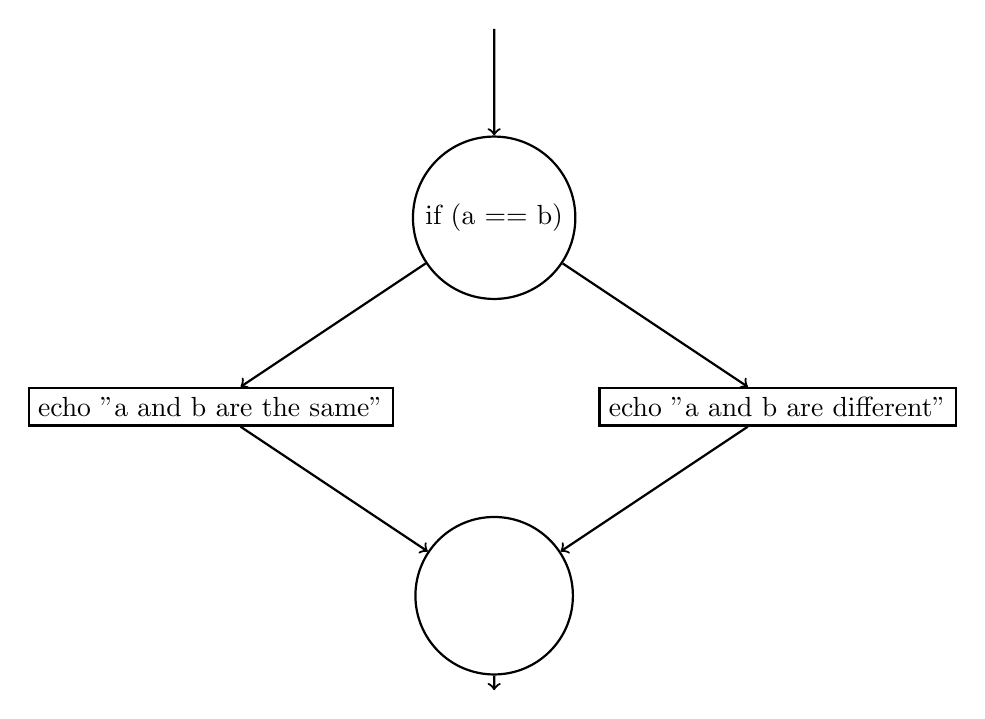
\begin{tikzpicture}[thick,scale=0.6, every node/.style={scale=0.6}]

\begin{scope}[every node/.style={circle,thick,draw}]
\node (node 1) at (4,8) {if (a == b)};
\node[rectangle] (node 2) at (-2,4) {echo "a and b are the same"};
\node[rectangle] (node 3) at (10,4) {echo "a and b are different"};
\node[circle,minimum size=2cm] (node 4) at (4,0) {}; 
\end{scope}

\begin{scope}
\draw [->] (4,12) -- (node 1);
\path [->] (node 1) edge node[right] {} (node 2);
\path [->] (node 2) edge node[right] {} (node 4);
\path [->] (node 1) edge node[right] {} (node 3);
\path [->] (node 3) edge node[right] {} (node 4);
\draw [->] (node 4) -- (4,-2);

\end{scope}

\end{tikzpicture} 

\caption{Control Flow Graph}
\label{fig:CFG}
\end{figure} 


There are different kinds of tools available for doing static code analysis such as IDE notifications, IDE tools, Dedicated tools, Linters and CLI tools. Out of which, the Dedicated tools and CLI tools are more likely to report security vulnerabilities, whereas others are more likely to report coding style issues. In this thesis, we will look into the usability aspect of such tools. 


\section{Usability}

The Human Computer Interaction researcher, Dr. Jakob Nielsen defines Usability as "a quality attribute that assesses how easy user interfaces are to use" \cite{usability-define}. It is characterised by five quality elements:

\begin{enumerate}
\item \textbf{Learnability:}  It says whether the design is simple for the person seeing the design for the first time and he can understand it.
\item \textbf{Efficiency:}  After getting familiar with design, how simple it is to do the tasks in a shorter time as possible?
\item \textbf{Memorability:} Once the person knew the design and worked for some time. Later, when he comes back after some significant time then is the design helpful enough to memorise?
\item \textbf{Errors:} It signifies the possibility of a person encountering the design do some errors and then whether he could recover from it easily or not.
\item \textbf{Satisfaction:} It determines the delightfulness of the person using the design.
\end{enumerate}

\section{Wireframe}

A wireframe is a methodology of showing a blueprint of a certain product. For example, if we consider to Wireframe a User Interface of an Application. It means to show a blueprint design of how the Application UI look like with different elements like buttons, text boxes etc placed on it and also how they interact and navigate to other User Interfaces. The blueprint design could vary from low fidelity i.e., rough sketches to high fidelity i.e., a more closer look to the desired final UI. There are several tools available in the market to do Wireframe and Balsamiq \cite{B} is one such tool. It is a kind of prototyping the actual product with certain simulation in functionality and visualization of the actual product. The advantage of this is the easiness of finding the mistakes in design earlier and so the cost of fixing them would be less. Here is an example of Wireframe done to a website idea about how it should look and the elements I would like to see as on a end product i.e., final front-end  design of the website coded is shown in the following \autoref{fig:wireframe_website} of what one could design using Balsamiq tool and discuss with peers how they feel or to oneself to draw the ideas of what they want to achieve before actually coding to get the web page with the desired UI. \\ \\

\begin{figure}[hbt!]
	\centering
	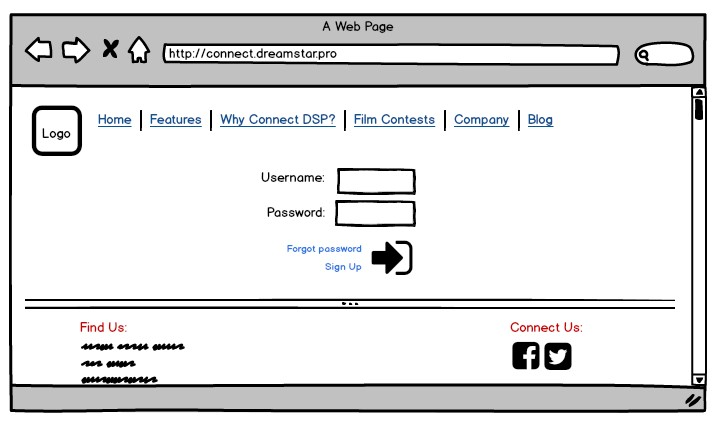
\includegraphics[width=\linewidth]{figures/Connect_DSP}
	\caption{An Example to Wireframe a Website.\cite{B}}
	\label{fig:wireframe_website}
\end{figure}

\section{User Experience Design} 
\label{sec:uxd}

User Experience ( UX ) Design plays a vital role in the success of a product but often underestimated. In a typical software industry, they say reasons to like it might lead to over budget or no time in order to skip it and get right into the development phase. Well, a User Experience Design process is far beyond what we know as User Interface Design or Usability.  User Interface Design is what typically done by Wireframe tool and Usability is a way of testing whether the designed product is usable enough or not. A User Experience ( UX ) Design is a user-centered process which emphasis on the context of the user and his needs than rather focusing solely on interface design. \cite{UX} For example, let us say you designed a navigation application where the user says I want to reach from point A to point B and it displays the route. Now, what if the user wants to mention points as a market name instead of street name and your underlying database consists only street names, that is a bad user experience ( UX ) even though the application is designed with better UI and also Usable. Its Design \cite{UXD} cycle as seen in the \autoref{fig:ux-design} illustrates an iterative cycle where the requirements are gathered, then a prototype is made on it and evaluated, then again new requirements are gathered based on the evaluation. \\ \\

\begin{figure}[hbt!]
	\centering
	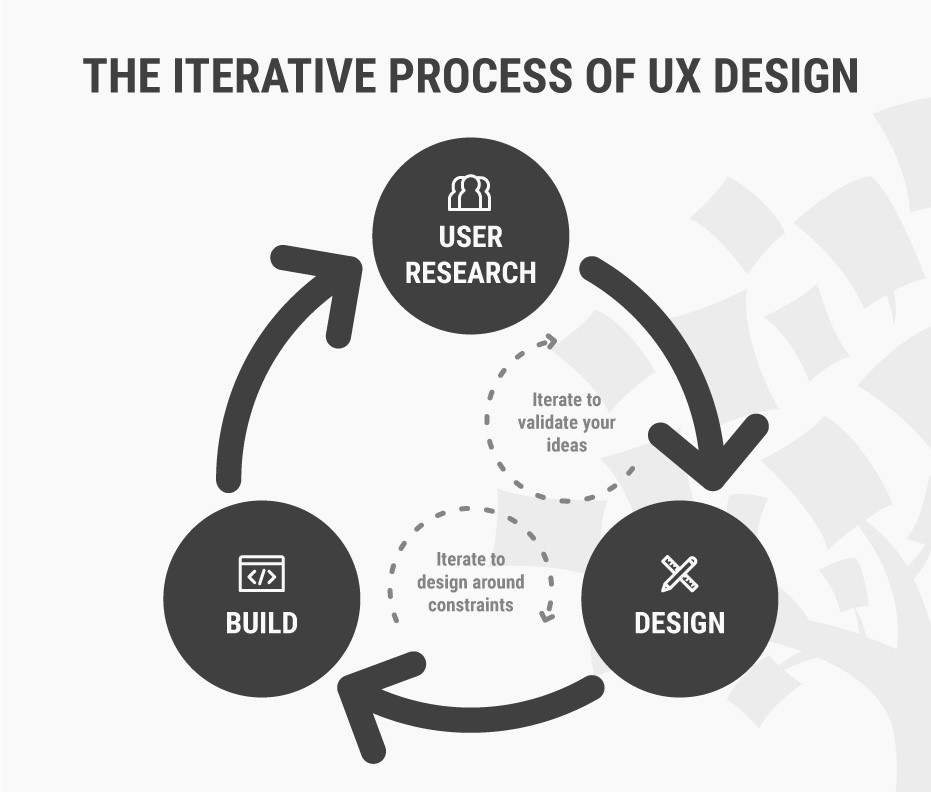
\includegraphics[width=\linewidth]{figures/ux-design}
	\caption{UX-Design.\cite{UXD}}
	\label{fig:ux-design}
\end{figure}

The applicability of the User Experience Design can be seen in detail at \autoref{ch:approaches}. 



\let\cleardoublepage\clearpage